\documentclass[a4paper,12pt]{article}

% ---------------------------
% PACKAGES
% ---------------------------
\usepackage[utf8]{inputenc}       % UTF-8 encoding for special characters
\usepackage[T1]{fontenc}          % Better font encoding for PDF output
\usepackage[ngerman,english]{babel} % Support for German and English text
\usepackage{graphicx}             % For including images
\usepackage{caption}              % For better figure and table captions
\usepackage{booktabs}             % For professional-looking tables
\usepackage{hyperref}             % For clickable references in PDF
\usepackage{tocloft}              % To customize TOC, LOF, LOT
\usepackage{geometry}             % To control margins and page layout
\usepackage{setspace}             % For line spacing
\usepackage{titlesec}             % For better section title formatting
\usepackage{csquotes}             % Recommended for correct localized quotation marks
\usepackage[style=ieee]{biblatex} % IEEE citation style
\addbibresource{sources.bib}      % <-- Your bibliography file
\graphicspath{{images/}}          % Folder for images
\geometry{margin=2.5cm}           % Page margins
\onehalfspacing                   % 1.5 line spacing

% ---------------------------
% DOCUMENT START
% ---------------------------
\begin{document}

% ---------------------------
% TITLE PAGE
% ---------------------------
\begin{titlepage}
    \centering
    {\Huge \textbf{Titel des Dokuments}\par}
    \vspace{2cm}
    {\Large Autor: Max Mustermann\par}
    {\large Version: 1.0\par}
    {\large Datum: \today\par}
    \vfill
    {\large Universität Musterstadt \\ Fakultät für Informatik}
\end{titlepage}

% ---------------------------
% VERSION HISTORY PAGE
% ---------------------------
\section*{Versionshistorie}
\begin{tabular}{lllp{8cm}}
\toprule
\textbf{Version} & \textbf{Datum} & \textbf{Autor} & \textbf{Änderung} \\
\midrule
1.0 & \today & Max Mustermann & Erstfassung des Dokuments \\
\bottomrule
\end{tabular}
\newpage

% ---------------------------
% ABSTRACT
% ---------------------------
\selectlanguage{english}
\begin{abstract}
This document demonstrates how to create a professional LaTeX structure in VS Code. 
It includes examples for title pages, figures, tables, references, quotations, and automatic lists.
\end{abstract}
\selectlanguage{ngerman}
\newpage

% ---------------------------
% TABLES OF CONTENTS, FIGURES, TABLES
% ---------------------------
\tableofcontents
\newpage
\listoffigures
\newpage
\listoftables
\newpage

% ---------------------------
% MAIN CONTENT
% ---------------------------

\section{Einleitung}
Dies ist die Einleitung. Hier wird ein Beispieltext mit einer Quelle zitiert \cite{ieee_example}. 

% Example of a direct quotation using csquotes:
Wie in \textquote{John Doe and Jane Smith zeigen in ihrer Arbeit, dass strukturierte Dokumente die Lesbarkeit erheblich verbessern}~\cite{ieee_example} beschrieben, 
ist die Nutzung von \LaTeX{} für akademische Arbeiten weit verbreitet.

\subsection{Motivation}
Hier könnte Ihre Motivation stehen. Nutzen Sie Absätze, um Ihre Ideen klar zu strukturieren.

\subsubsection{Hintergrund}
Unterabschnitt dritter Ebene (z. B. 1.1.1) – Hier können Sie detaillierte technische Hintergründe beschreiben.

\subsubsection{Hintergrund2}
Unterabschnitt dritter Ebene (z. B. 1.1.2) – Weitere Details oder Unterthemen.

% ---------------------------
% FIGURE EXAMPLE
% ---------------------------
\section{Beispiel mit Bildern und Tabellen}

\subsection{Abbildung}
Abbildung~\ref{fig:example} zeigt ein Beispielbild.

\begin{figure}[h!]
    \centering
    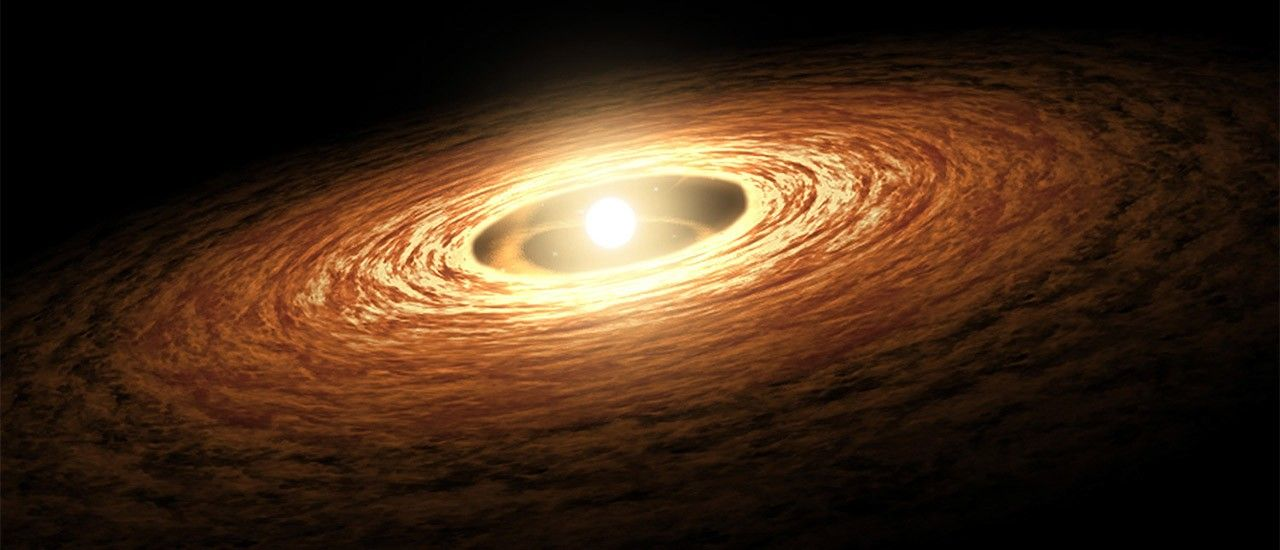
\includegraphics[width=0.6\textwidth]{universe} % Replace 'universe' with your actual image file
    \caption{Beispielhafte Abbildung}
    \label{fig:example}
\end{figure}

% ---------------------------
% TABLE EXAMPLE
% ---------------------------
\subsection{Tabelle}
Tabelle~\ref{tab:example} zeigt eine einfache Tabelle.

\begin{table}[h!]
    \centering
    \begin{tabular}{lll}
        \toprule
        Spalte 1 & Spalte 2 & Spalte 3 \\
        \midrule
        A & B & C \\
        D & E & F \\
        \bottomrule
    \end{tabular}
    \caption{Beispielhafte Tabelle}
    \label{tab:example}
\end{table}

% ---------------------------
% CONCLUSION
% ---------------------------
\newpage
\section{Fazit}
Hier steht das Fazit. Weitere Quellenangaben sind in Abschnitt~\ref{sec:references} zu finden.

% ---------------------------
% BIBLIOGRAPHY
% ---------------------------
\newpage
\section{Quellenverzeichnis}
\label{sec:references}
\printbibliography

\end{document}
